% =====================================================================
% FORM-AC-01 — Análisis de caso: fallo real en un sistema distribuido
% Caso: caída de Cloudflare del 21 de junio de 2022
% Equipo ALM — Aplicaciones Distribuidas (ISR-701), UTEQ
%
% Compilar con pdfLaTeX + Biber:
%   pdflatex main.tex
%   biber main
%   pdflatex main.tex
%   pdflatex main.tex
% (o simplemente: latexmk -pdf main.tex)
%
% Límite del enunciado: el cuerpo (apartados 1 a 6) ocupa como máximo
% 2 páginas, sin contar la carátula ni las referencias.
% =====================================================================
\documentclass[11pt,a4paper]{article}

\usepackage[T1]{fontenc}
\usepackage[utf8]{inputenc}
\usepackage[spanish,es-tabla,es-nodecimaldot]{babel}
\usepackage{mathptmx}
\renewcommand{\ttdefault}{lmtt}
\usepackage[a4paper,margin=2cm]{geometry}
\usepackage{microtype}
\usepackage{graphicx}
\usepackage{array,booktabs,tabularx}
\usepackage{caption}
\usepackage{enumitem}
\usepackage{titlesec}
\usepackage[autostyle=false,style=english]{csquotes}
\usepackage[backend=biber,style=ieee,maxbibnames=2,minbibnames=1,urldate=long]{biblatex}
\addbibresource{referencias.bib}
\usepackage{xpatch}
% Páginas web sin fecha: "(s. f.)" en lugar de "()"
\xpatchbibdriver{online}
  {\printtext[parens]{\usebibmacro{date}}}
  {\iffieldundef{year}{\printtext[parens]{\bibstring{nodate}}}{\printtext[parens]{\usebibmacro{date}}}}
  {}{\PackageWarning{main}{No se pudo ajustar el driver online}}
\usepackage[hidelinks]{hyperref}
\usepackage{xurl}

% --- Datos de la entrega (si el repo cambia de nombre o de cuenta, se cambia aquí) ---
\newcommand{\repourl}{https://github.com/Washinton-Apunte/FORM-AC-01-Cloudflare-2022-ALM}

% --- Formato compacto para respetar las 2 páginas ---
\setlength{\parindent}{0pt}
\setlength{\parskip}{2pt plus 1pt}
\titleformat{\section}{\normalfont\large\bfseries}{\thesection.}{0.5em}{}
\titlespacing*{\section}{0pt}{6pt}{2pt}
\captionsetup{font=small,labelfont=bf,labelsep=period,skip=3pt}
\captionsetup[table]{position=above}
\setlist[itemize]{nosep,leftmargin=*}
\newcolumntype{L}{>{\raggedright\arraybackslash}X}
\renewcommand{\arraystretch}{1.05}
\setlength{\textfloatsep}{8pt plus 2pt minus 2pt}
\setlength{\intextsep}{6pt plus 2pt minus 2pt}

% --- Ajustes IEEE en español: "et al." en cursiva, "pp.", guion largo en rangos ---
\DefineBibliographyStrings{spanish}{%
  andothers = {\mkbibemph{et~al\adddot}},
  pages     = {pp\adddot},
  page      = {p\adddot},
  url       = {disponible en},
  urlseen   = {consultado el},
}
\DefineBibliographyExtras{spanish}{\protected\def\bibrangedash{\textendash\penalty\hyphenpenalty}}

\begin{document}

% ---------------------------------------------------------------------
% CARÁTULA (no cuenta para las 2 páginas)
% ---------------------------------------------------------------------
\begin{titlepage}
  \centering
  \begin{minipage}[c]{0.17\textwidth}\centering
    
\includegraphics[height=2.9cm]{img/logo-uteq.png}
  \end{minipage}%
  \hfill
  \begin{minipage}[c]{0.62\textwidth}\centering
    {\Large\bfseries UNIVERSIDAD TÉCNICA ESTATAL\\[2pt] DE QUEVEDO\par}
    \vspace{0.3cm}
    {\large\bfseries Facultad de Ciencias de la Computación\\[1pt] y Diseño Digital\par}
    \vspace{0.2cm}
    {\large\itshape Carrera de Software\par}
  \end{minipage}%
  \hfill
  \begin{minipage}[c]{0.17\textwidth}\centering
    
\includegraphics[height=2.7cm]{img/logo-facultad.png}
  \end{minipage}
  \par\vspace{1.6cm}
  {\Large\bfseries Aplicaciones Distribuidas (ISR-701)\par}
  \vspace{0.3cm}
  {\large FORM-AC-01 — Análisis de caso: fallo real en un sistema distribuido\par}
  \vspace{1.6cm}
  {\LARGE\bfseries Caída de Cloudflare del 21 de junio de 2022:\\[2pt]
   retiro de prefijos BGP en 19 centros de datos\par}
  \vspace{1.8cm}
  {\large\bfseries Equipo ALM\par}
  \vspace{0.3cm}
  {\large Apunte Pazmiño Washington German\\
          Loor Suarez Jordan Josue\\
          Macias Vasquez Cesar Abrahan\par}
  \vfill
  \begin{tabular}{@{}rl@{}}
    \textbf{Docente:}          & Gleiston Guerrero Ulloa, PhD \\
    \textbf{Nivel y paralelo:} & Séptimo nivel, paralelo B \\
    \textbf{Semana:}           & 3 (9 al 15 de noviembre de 2026) \\
    \textbf{Fecha de entrega:} & 15 de noviembre de 2026 \\
  \end{tabular}
  \par\vspace{0.8cm}
  \textbf{Repositorio:} \url{\repourl}
  \par\vspace{0.4cm}
  Quevedo, Ecuador
\end{titlepage}

% ---------------------------------------------------------------------
% CUERPO (apartados 1 a 6, máximo 2 páginas)
% ---------------------------------------------------------------------
\pagenumbering{arabic}
\setcounter{page}{1}
\label{inicio-cuerpo}


\section{Descripción del incidente}

El 21 de junio de 2022, Cloudflare presentó una caída
en parte de su red debido a un error en la configuración
del enrutamiento BGP, que se utiliza para dirigir el
tráfico de Internet. Este problema afectó a 19 centros
de datos y provocó que varios sitios web y servicios
que dependían de Cloudflare dejaran de estar disponibles.
La interrupción comenzó a las 06:27 UTC y los centros
afectados lograron recuperarse a las 07:42 UTC, por lo
que el problema duró aproximadamente 75 minutos
\cite{cloudflare2022}.

\textbf{Línea de tiempo (21 de junio de 2022, UTC), según el informe oficial de Cloudflare \cite{cloudflare2022}:}
\begin{itemize}
    \item \textbf{03:56:} Cloudflare inició la implementación
    de un cambio en su red.
    \item \textbf{06:17:} El cambio llegó a centros de datos
    que manejaban una gran cantidad de tráfico.
    \item \textbf{06:27:} Se produjo la caída de los 19
    centros de datos afectados.
    \item \textbf{06:32:} Cloudflare reconoció el incidente
    y comenzó a investigarlo.
    \item \textbf{06:58:} Se encontró la causa del problema
    y se empezó a revertir el cambio.
    \item \textbf{07:42:} Los centros afectados volvieron
    a funcionar con normalidad.
    \item \textbf{08:00:} Cloudflare dio por finalizado
    el incidente.
\end{itemize}

\section{Causas raíz}
Como se detalla en el diagrama de Ishikawa (Figura \ref{fig:ishikawa}), la interrupción no fue producto de un ciberataque (síntoma), sino de un fallo de configuración interno. La causa raíz técnica se originó durante la transición a la nueva arquitectura Multi-Colo PoP (MCP), cuando un error operativo al reordenar los términos de las políticas de enrutamiento BGP provocó el retiro involuntario de prefijos de red críticos en los enrutadores perimetrales \cite{cloudflare2022}.

\begin{figure}[htbp]
    \centering
    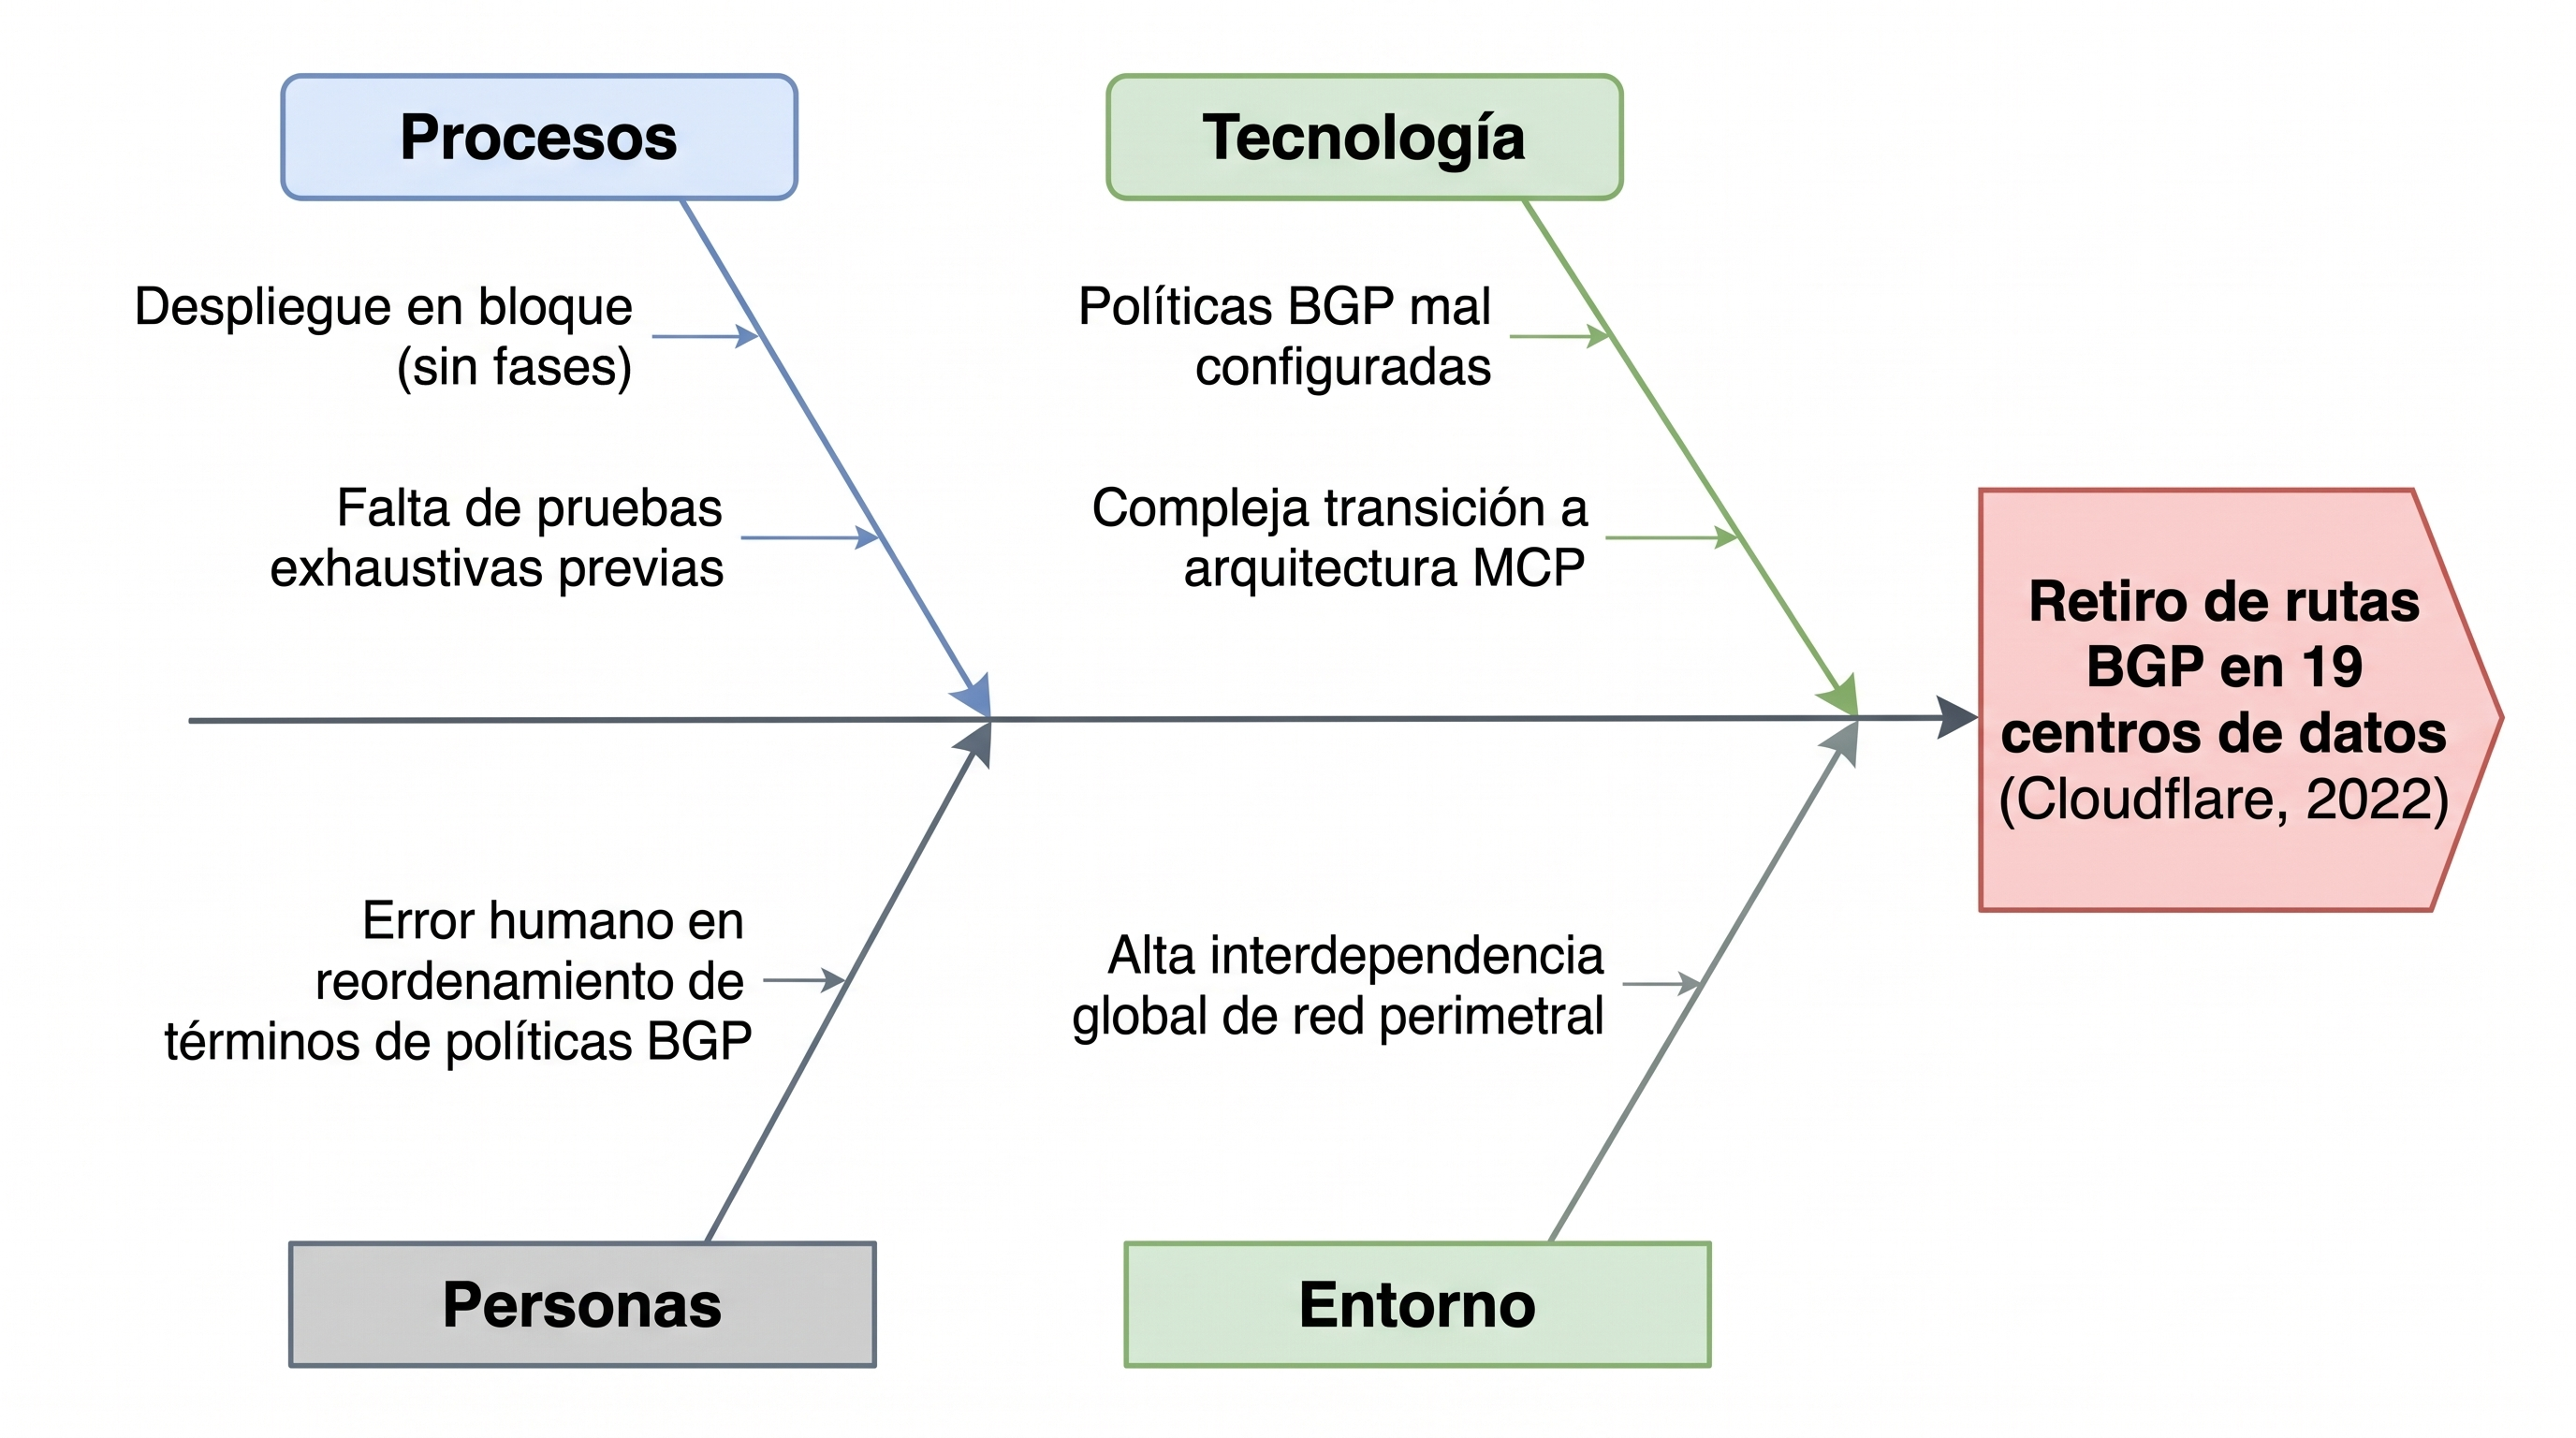
\includegraphics[width=\textwidth]{diagramas/ishikawa-cloudflare-2022}
    \caption{Diagrama de Ishikawa elaborado por el equipo con las causas del incidente.}
    \label{fig:ishikawa}
\end{figure}

\section{Impacto cuantificado}
El incidente desconectó 19 centros de datos (4\% del total de la red de Cloudflare), los cuales atienden el 50 \% de las solicitudes HTTP
globales \cite{cloudflare2022}. La interrupción duró aproximadamente 75 minutos y afectó a diversas plataformas dependientes, 
como GitLab \cite{gitlab2022incident} y Acquia \cite{acquia2022incident}. Este tiempo de inactividad incumple directamente el SLA Business, 
el cual garantiza un 100\% de disponibilidad y ofrece como único remedio créditos de servicio a los clientes afectados \cite{cloudflare2026sla}.

% Apartado 4 — Responsable: Apunte Pazmiño Washington German
\section{Relación con la Unidad 1}\label{sec:unidad1}

\textbf{Transparencia.} Se rompió la transparencia de fallos: según su definición, el usuario no debería notar el fallo y el sistema tendría que recuperarse solo~\cite{vansteen2016brief}. Pasó lo contrario: en algunas regiones no se podía entrar a sitios que usan Cloudflare, mientras que en otras todo funcionaba con normalidad. Tampoco hubo recuperación automática: los ingenieros tuvieron que revertir el cambio y todo volvió a la normalidad recién a las 07:42 UTC~\cite{cloudflare2022}.

\textbf{Teorema CAP.} Sí hubo una partición, pero provocada por una configuración y no por un cable cortado: al dejar de anunciarse los prefijos BGP \emph{site-local}, los servidores de los 19 centros ya no se alcanzaban entre sí ni llegaban a los servidores de origen de los clientes~\cite{cloudflare2022}. Ante una partición hay que elegir: responder con datos desactualizados (se pierde la consistencia) o no responder (se pierde la disponibilidad)~\cite{gilbert2002brewer}. Pasó lo segundo: se sacrificó la disponibilidad, aunque nadie lo eligió. El informe no menciona pérdida de datos~\cite{cloudflare2022}.

\textbf{Tolerancia a fallos.} Debía proteger el despliegue escalonado, junto con la prueba en seco y la revisión por pares, pero ninguno detectó el error: el escalonado no incluyó un centro MCP hasta el último paso, así que el cambio llegó de golpe a los \emph{spines} de los 19 centros~\cite{cloudflare2022}. La malla de \emph{spines} tampoco ayudó: la redundancia cubre fallos independientes, no una mala configuración copiada en todos. Esto coincide con Govindan \emph{et al.}: en la mayoría de los fallos graves que analizaron en la red de Google había una operación de gestión en curso~\cite{govindan2016evolve}.


\section{Mitigación aplicada por Cloudflare}

Para recuperar el servicio, los ingenieros de Cloudflare
utilizaron procedimientos de acceso de respaldo, ya que
el fallo también dificultaba la conexión con los centros
afectados. Una vez identificada la causa, comenzaron a
revertir la configuración incorrecta de los routers.
La recuperación fue gradual y, a las 07:42 UTC, los
19 centros de datos afectados estaban nuevamente
operativos \cite{cloudflare2022}.

Después del incidente, Cloudflare anunció mejoras en
sus procedimientos. Entre ellas, realizar pruebas en
centros con arquitectura MCP antes de extender los
cambios, revisar las reglas de enrutamiento para evitar
errores en su orden y automatizar la reversión de
configuraciones cuando se detecten problemas.
Estas medidas buscan reducir el impacto de futuros
fallos y acelerar la recuperación del servicio
\cite{cloudflare2022}.


\section{Lecciones aprendidas para el PFC (SREI)}

El incidente de Cloudflare demuestra que una
configuración incorrecta, un despliegue sin controles
y la falta de reversión pueden afectar varios servicios
al mismo tiempo \cite{cloudflare2022}. En SREI
identificamos tres riesgos relacionados con las
tecnologías que utilizamos y las medidas que
incorporaremos en TA-PFC-E1.

\begin{table}[htbp]
\centering
\small
\begin{tabularx}{\linewidth}{@{}L L@{}}
\toprule
\textbf{Riesgo en SREI} & \textbf{Medida preventiva} \\
\midrule
Una configuración incorrecta de la conexión entre
Angular y Spring Boot podría impedir que los usuarios
accedan a las funciones del sistema.
&
Verificar las direcciones y configuraciones de conexión
en un entorno de pruebas antes de publicar cambios.
\\
\addlinespace
Una actualización del backend Spring Boot o de las
tablas de PostgreSQL podría provocar errores en el
registro y consulta de eventos.
&
Probar las actualizaciones y migraciones antes de
aplicarlas, conservando respaldos de la base de datos.
\\
\addlinespace
Un cambio en Docker Compose podría afectar
simultáneamente los contenedores y dejar SREI
fuera de servicio.
&
Probar los cambios antes del despliegue, actualizar
los servicios de forma controlada y conservar las
versiones anteriores para facilitar la reversión.
\\
\bottomrule
\end{tabularx}
\end{table}


\label{fin-cuerpo}

% ---------------------------------------------------------------------
% REFERENCIAS, DECLARACIÓN DE IA Y OBSERVACIONES (fuera de las 2 páginas)
% ---------------------------------------------------------------------
\clearpage
\printbibliography[title={Referencias}]

% Declaración de uso de IA — Responsable: Apunte Pazmiño Washington German
% Tiene que decir lo que realmente pasó. Si alguien aclara otro uso de IA, se agrega aquí.
\section*{Declaración de uso de inteligencia artificial}

\begingroup\footnotesize
\textbf{Herramientas de apoyo:} Claude (Anthropic; modelos Opus 5.5 y Sonnet 5.5), consultado el 14 y 15 de noviembre de 2026, y ChatGPT (OpenAI), utilizado como asistente por Jordan Loor.

\textbf{Uso como herramienta de asistencia en el trabajo del equipo:}
\begin{itemize}
\item \textbf{Apoyo en verificación bibliográfica:} asistencia para contrastar metadatos en Crossref (autores, título, revista, páginas y DOI) a partir de las fuentes localizadas por el equipo.
\item \textbf{Revisión de estilo y maquetación:} sugerencias de corrección ortográfica, gramatical y de sintaxis en formato LaTeX.
\item \textbf{Estructuración técnica:} apoyo en la organización de la plantilla LaTeX, el archivo README y la estandarización de comandos de git para el flujo de trabajo del equipo.
\item \textbf{Asistencia de formato:} apoyo en la depuración de etiquetas XML para el diagrama de Ishikawa en draw.io y revisión preliminar de estructura para los apartados 2 y 3.
\end{itemize}

\textbf{Autoría y participación de cada integrante:}
\begin{itemize}
\item \textbf{Washington Apunte:} realizó la lectura crítica de las fuentes y redactó íntegramente el apartado 4. Utilizó Claude únicamente como apoyo para revisar el estilo de redacción, contrastar cifras contra el informe oficial y depurar el formato LaTeX de las citas.
\item \textbf{Jordan Loor:} investigó y redactó los apartados 1, 5 y 6, así como las observaciones. Empleó ChatGPT como herramienta de consulta para pulir la cohesión de la descripción del incidente, validar la estructura de las medidas de mitigación y riesgos de SREI definidos por él, y verificar la sintaxis LaTeX antes de integrar su aporte.
\item \textbf{César Macías:} desarrolló el análisis y el contenido de los apartados 2 y 3, así como el diseño conceptual del diagrama de Ishikawa, apoyándose en la IA para optimizar la sintaxis del código fuente (XML) en draw.io y la estructura base. Ejecutó manualmente la exportación de los archivos \texttt{.drawio} y \texttt{.pdf}, la limpieza y organización del repositorio y las correcciones técnicas en LaTeX (SLA Business y la precisión sobre el ciberataque).
\end{itemize}
\endgroup

\section*{Observaciones y cambios realizados}

El caso no se expuso en clase, debido a que el docente
no programó una presentación para esta actividad.
Por este motivo, hasta el cierre del 15 de noviembre
de 2026, el equipo ALM no recibió evaluaciones entre
pares ni observaciones escritas del docente.

Si se reciben observaciones posteriormente, se
registrarán en esta tabla junto con los cambios
realizados o la justificación correspondiente.

\begin{table}[htbp]
\centering
\small
\begin{tabularx}{\linewidth}{@{}L L@{}}
\toprule
\textbf{Observación recibida} &
\textbf{Cambio realizado o justificación} \\
\midrule
No se recibieron observaciones hasta el cierre
de la actividad.
&
No se realizaron cambios por retroalimentación,
ya que no hubo evaluaciones ni observaciones recibidas. \\
\bottomrule
\end{tabularx}
\end{table}


\end{document}
